\documentclass{article}

\usepackage{amsmath,amsthm,amsfonts,amssymb,bm}
\addtolength{\textheight}{5.0cm}
\addtolength{\voffset}{-3.5cm}
\addtolength{\hoffset}{-2.5cm}
\addtolength{\textwidth}{4.0cm}

%\allowdisplaybreaks

%\usepackage{subeqnarray}
%\usepackage{mathrsfs}
%\usepackage{color}
%\usepackage{url}
%\usepackage{ulem}
\usepackage{indentfirst}
%\usepackage{textcomp}
%\usepackage{graphics}
%\usepackage{graphicx}
%\usepackage[hang,small,bf]{caption}
%\setlength{\captionmargin}{50pt}


%\usepackage{tikz}
%\usetikzlibrary{mindmap,trees}
\usepackage{graphicx}
%\usepackage[hang,small,bf]{caption}
%\setlength{\captionmargin}{50pt}



\begin{document}
\title{Power Spctrum \& Its Evolution}
\author{MA Lei}
%\maketitle

\begin{itemize}

\item
{\bf I can't get a plot exactly the same as figure1(a).}

I used the following parameters.

\begin{eqnarray*}
&&\Omega _{\text{DE0}}=0.734;\Omega _{\text{k0}}=0;\Omega _{\text{m0}}=0.1334\left/\left(0.71^2\right)\right.;\Omega _{\text{r0}}=8.09*10^{-5};\\
&&h=0.71;H_0=\frac{100 h}{300000};
\end{eqnarray*}

The Hubble equations are
\begin{eqnarray}
H_s[\text{a$\_$}]&=&\text{Hs0} \sqrt{\frac{\Omega _{\text{m0},s}}{a^3}+\frac{\Omega _{\text{r0},s}}{a^4}}\\
H_L[\text{a$\_$}]&=&\text{HL0} \sqrt{\Omega _{\text{DE0}}+\frac{\Omega _{\text{m0}}}{a^3}+\frac{\Omega _{\text{r0}}}{a^4}}\\
H_d[\text{a$\_$}]&=&\text{Hd0} \sqrt{\frac{\Omega _{\text{DE0}}}{a^{1.5}}+\frac{\Omega _{\text{m0}}}{a^3}+\frac{\Omega _{\text{r0}}}{a^4}}
\end{eqnarray}
in which, subscripts $_s,_L,_d$ denote stand CDM, LCDM, DE(with $w=-0.5$) respectively.

Using these equations and three points on figure2(a), we find
\begin{eqnarray}
H_s\left[10^{-6}\right]&=&H_L\left[10^{-6}\right]\\
H_s[1]&=&1.25H_L[1]\\
H_s[0.3]&=&1.9H_L[0.3]
\end{eqnarray}

After simplifying, they become
\begin{eqnarray}
\text{Hs0}^2 \left(1.\times 10^{18} \Omega _{\text{m0},s}+1.\times 10^{24} \Omega _{\text{r0},s}\right)=4.54612\times 10^{12} \\
\text{Hs0}^2 \left(\Omega _{\text{m0},s}+\Omega _{\text{r0},s}\right)=\text{8.740454543229165$\grave{ }$*${}^{\wedge}$-8}\\
\text{Hs0}^2 \left(37.037 \Omega _{\text{m0},s}+123.457 \Omega _{\text{r0},s}\right)==\text{2.132220394599451$\grave{ }$*${}^{\wedge}$-6}
\end{eqnarray}

To see this more easily, we change the arguments, $Hs0\rightarrow x, \Omega_{m0.s}\rightarrow x, \Omega_{r0,s}\rightarrow z$, the equations are
\begin{eqnarray}
x^2 \left(y+10^6 z\right)&=&4.546121111111111*10^{-6}\\
x^2 (y+z)&=& 8.740454543229165* 10^{-8}\label{eqarray_2}\\
x^2 (y+3.33333 z)&=& 5.7569950654185174*10^{-8} \label{eqarray_3}
\end{eqnarray}

From equation \ref{eqarray_2} and \ref{eqarray_3}, we can find that there won't be any positive solutions.

The key point is that the last term in \ref{eqarray_3} should be larger than that of \ref{eqarray_2}. This lead to the fact that the ratio value in figure2(a) at $1+z\sim 3.3$ should be larger than 2.3 if the value at $1+z=1$ is 1.25, as the figure shows.

This evalution indicates that the parameters of LCDM used to generate figure2(a) is very different from the one I am using, which is extracted from the WMAP7 year data.
In principal, I can always fit all the values from this figure. Anyhow, this is stupid to do so and this is not easy because the radiation part is small.






\item

{\bf As for figure2(a), here is the problem.}

\begin{figure}[!htpb]
\centering
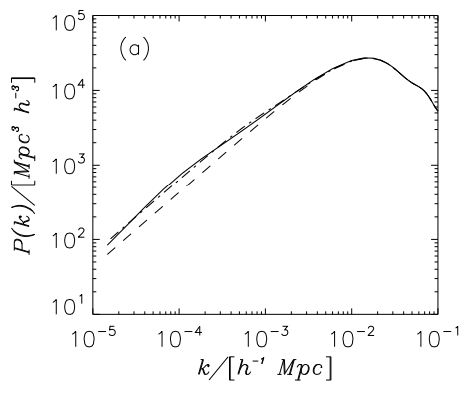
\includegraphics[width=350pt]{figure2_a.jpg}
\caption{Figure2(a) in arxiv:1109.4038}\label{fig:figure2_a}
\end{figure}

This figure is the power spectrum of matter,in which "matter power spectra of the concordance $\Lambda$CDM (dashed line) and the fiducial DE model (dot-dashed line)" and "the solid line represents the approximated DE power spectrum derived from the $\Lambda$CDM one".

There are two things to be explained.

The first one is that the $k<0.0003$ perturbations are outside of the horizon nowaday. So all the modes with $k<0.0003$ has the same amplitude of matter density $\delta_m$ according to the assumaption. Since the power is $P\sim \frac{\delta^2}{k^{3}}$, the line goes up when k runs to the smaller value.

The second one is 



I have no idea with the descending of the line in figure2(a).






\item
{\bf I think we shouldn't use the formulas (12) and (13) in their paper.}

The assumption that the primordinal matter perturbation $\delta_i$ (or potential perturbation $\Phi_i$) are the same is not a substantial point, since this $\delta_i$ gives us the freedom of renormalizing the power spectrum.

It's better to start over. the matter perturbation at any $a$ is
\[
\delta_m(a)=\delta_i \frac{1}{D_+(a_i)}D_+(a)
\]
where $\delta_i$ is the initial perturbation, $D_+$ is the growth factor, $a_i$ is the scale factor at intial.

Then the $Q$ factor should be defined as
\[
Q=\frac{\delta_i^X D_+^X(a)/D_+^X(a_i)}{\delta_i^F D_+^F(a)/D_+^F(a_i)}
\]

Their work take the condition that $\delta_i^X=\delta_i^L$. However, this leaves us no parameters for the normalization of power spectrum. If we keep $\delta_i^X$ and $\delta_i^L$, then we can change these to adjust the power spectrum.

Their paper did not metion where the freedom of renormalization comes from.





\end{itemize}









\end{document}